% Exercices de la première passe « Approche cinématique ».
% Le titre et le label de la partie exercices sont créés par le document maître.

\begingroup
% Couche d'intégration de la conversion Word/Pandoc du cours de cinématique.
% Elle ne modifie pas contenu.tex : les corrections sont appliquées en mémoire.

\makeatletter
\let\TLFourKOriginalIncludeGraphics\includegraphics
\newif\ifTLFourKVectorGraphic

\newcommand{\TLFourKMissingGraphic}[1]{%
  \begin{tikzpicture}[baseline=(current bounding box.center)]
    \node[
      draw=TLCoverBlue!55,
      rounded corners=1mm,
      fill=TLCoverBlue!4,
      text=TLCoverBlue!80!black,
      align=center,
      font=\sffamily\scriptsize,
      inner sep=2mm,
      text width=25mm
    ] {Illustration vectorielle\\non convertie\\\ttfamily #1};
  \end{tikzpicture}%
}

\newcommand{\TLFourKPlaceOriginal}[3]{%
  \ifinner
    \ifdim\linewidth<12mm
      \TLFourKOriginalIncludeGraphics[width=8mm,height=8mm,keepaspectratio]{#3}%
    \else
      \adjustbox{max width=.92\linewidth,max totalheight=.68\textheight}{%
        \IfBooleanTF{#1}
          {\TLFourKOriginalIncludeGraphics*[#2]{#3}}
          {\TLFourKOriginalIncludeGraphics[#2]{#3}}%
      }%
    \fi
  \else
    \par\noindent
    \makebox[\linewidth][c]{%
      \adjustbox{max width=.95\linewidth,max totalheight=.76\textheight}{%
        \IfBooleanTF{#1}
          {\TLFourKOriginalIncludeGraphics*[#2]{#3}}
          {\TLFourKOriginalIncludeGraphics[#2]{#3}}%
      }%
    }%
    \par\noindent
  \fi
}

\newcommand{\TLFourKPlaceConverted}[1]{%
  \ifinner
    \ifdim\linewidth<12mm
      \TLFourKOriginalIncludeGraphics[width=8mm,height=8mm,keepaspectratio]{#1}%
    \else
      \adjustbox{max width=.92\linewidth,max totalheight=.68\textheight}{%
        \TLFourKOriginalIncludeGraphics[width=\linewidth,height=.70\textheight,keepaspectratio]{#1}%
      }%
    \fi
  \else
    \par\noindent
    \makebox[\linewidth][c]{%
      \adjustbox{max width=.95\linewidth,max totalheight=.76\textheight}{%
        \TLFourKOriginalIncludeGraphics[width=\linewidth,height=.74\textheight,keepaspectratio]{#1}%
      }%
    }%
    \par\noindent
  \fi
}

\RenewDocumentCommand{\includegraphics}{s O{} m}{%
  \begingroup
  \filename@parse{#3}%
  \edef\TLFourKGraphicExtension{\filename@ext}%
  \edef\TLFourKGraphicStem{\filename@area\filename@base}%
  \edef\TLFourKGraphicBase{\filename@base}%

  % Pictogrammes injectés dans des titres par Word/Pandoc. Les illustrations
  % utiles sont réinsérées après les titres par TLApplyCinematiquePatches.
  \ifboolexpr{
    test {\ifdefstring{\TLFourKGraphicBase}{image3}}
    or test {\ifdefstring{\TLFourKGraphicBase}{image7}}
    or test {\ifdefstring{\TLFourKGraphicBase}{image10}}
    or test {\ifdefstring{\TLFourKGraphicBase}{image52}}
    or test {\ifdefstring{\TLFourKGraphicBase}{image87}}
  }{%
    % rien
  }{%
    \TLFourKVectorGraphicfalse
    \ifdefstring{\TLFourKGraphicExtension}{emf}{\TLFourKVectorGraphictrue}{}
    \ifdefstring{\TLFourKGraphicExtension}{EMF}{\TLFourKVectorGraphictrue}{}
    \ifdefstring{\TLFourKGraphicExtension}{wmf}{\TLFourKVectorGraphictrue}{}
    \ifdefstring{\TLFourKGraphicExtension}{WMF}{\TLFourKVectorGraphictrue}{}

    \ifTLFourKVectorGraphic
      \IfFileExists{\TLFourKGraphicStem.png}{%
        \TLFourKPlaceConverted{\TLFourKGraphicStem.png}%
      }{%
        \IfFileExists{\TLFourKGraphicStem.pdf}{%
          \TLFourKPlaceConverted{\TLFourKGraphicStem.pdf}%
        }{%
          \IfFileExists{\TLFourKGraphicStem.jpeg}{%
            \TLFourKPlaceConverted{\TLFourKGraphicStem.jpeg}%
          }{%
            \ifinner
              \TLFourKMissingGraphic{\filename@base}%
            \else
              \par\noindent\makebox[\linewidth][c]{\TLFourKMissingGraphic{\filename@base}}\par\noindent
            \fi
          }%
        }%
      }%
    \else
      % Petite pastille de niveau utilisée dans les exercices.
      \ifdefstring{\TLFourKGraphicBase}{image101}{%
        \TLFourKOriginalIncludeGraphics[width=5mm,height=5mm,keepaspectratio]{#3}%
      }{%
        % Les deux illustrations de la règle du tire-bouchon sont réellement
        % prévues côte à côte.
        \ifdefstring{\TLFourKGraphicBase}{image11}{%
          \TLFourKOriginalIncludeGraphics[width=.28\linewidth,height=.18\textheight,keepaspectratio]{#3}\hfill
        }{%
          \ifdefstring{\TLFourKGraphicBase}{image12}{%
            \TLFourKOriginalIncludeGraphics[width=.28\linewidth,height=.18\textheight,keepaspectratio]{#3}\par\noindent
          }{%
            \TLFourKPlaceOriginal{#1}{#2}{#3}%
          }%
        }%
      }%
    \fi
  }%
  \endgroup
}

% Corrections sémantiques appliquées au contenu capturé.
\newcommand{\TLApplyCinematiquePatches}[1]{%
  % Illustrations retirées des signets/titres puis replacées dans le texte.
  \patchcmd{#1}
    {\label{cas-n2-prothuxe8se-transtibiale}}
    {\label{cas-n2-prothuxe8se-transtibiale}%
     \begin{center}\TLFourKOriginalIncludeGraphics[width=.34\linewidth,height=.25\textheight,keepaspectratio]{images/image7.jpeg}\end{center}}
    {}{}
  \patchcmd{#1}
    {\label{duxe9finition-du-produit-vectoriel}}
    {\label{duxe9finition-du-produit-vectoriel}%
     \begin{center}\TLFourKOriginalIncludeGraphics[width=.24\linewidth,height=.19\textheight,keepaspectratio]{images/image10.jpeg}\end{center}}
    {}{}
  \patchcmd{#1}
    {\label{vecteur-position}}
    {\label{vecteur-position}%
     \begin{center}\TLFourKOriginalIncludeGraphics[width=.20\linewidth,height=.16\textheight,keepaspectratio]{images/image52.png}\end{center}}
    {}{}
  \patchcmd{#1}
    {\label{cinuxe9matique-du-contact-ponctuel}}
    {\label{cinuxe9matique-du-contact-ponctuel}\TLContactPonctuel}
    {}{}

  % Le montage Word des quatre images du produit vectoriel est remplacé par
  % une figure TikZ lisible et réutilisable.
  \patchcmd{#1}
    {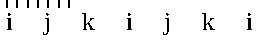
\includegraphics[width=\linewidth,height=.72\textheight,keepaspectratio]{images/image14.pdf}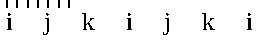
\includegraphics[width=\linewidth,height=.72\textheight,keepaspectratio]{images/image14.pdf}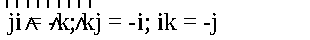
\includegraphics[width=\linewidth,height=.72\textheight,keepaspectratio]{images/image15.pdf}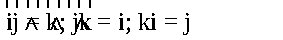
\includegraphics[width=\linewidth,height=.72\textheight,keepaspectratio]{images/image16.pdf}}
    {\TLProduitVectorielBase}
    {}{}

  % La loi trapèze est reconstruite en TikZ plutôt que conservée comme capture.
  \patchcmd{#1}
    {
\includegraphics[width=\linewidth,height=.72\textheight,keepaspectratio]{images/image94.png}}
    {\TLLoiTrapeze}
    {}{}
}
\makeatother


\CatchFileDef{\TLFourKSource}{contenu.tex}{}
\TLApplyCinematiquePatches{\TLFourKSource}

\long\def\TLFourKExtractExercises#1\subsection{Exercices du chapitre}\label{exercices-du-chapitre}#2\TLFourKStop{#2}

\small
\sloppy
\setlength{\tabcolsep}{4pt}
\renewcommand{\arraystretch}{1.08}
\setlength\LTleft{0pt}
\setlength\LTright{0pt}

\expandafter\TLFourKExtractExercises
  \TLFourKSource
  \TLFourKStop
\endgroup
